
\chapter{Plug-in Environment}
\label{cha:plug-in}

This chapter proposes a solution to the problem of extending U-Sem by adding custom functionality. Section \ref{sec:requirementsPlugin} identifies all functional and non-functional requirements that a successful solution must satisfy based on the problems discussed in Section \ref{sec:problemDefPlugin}. Section \ref{sec:approachPlugin} discusses the state of the art approaches and technologies that can contribute to solving the problem. Section \ref{sec:architecturePlugin} describes the architecture of U-Sem that we propose in order to solve the problem. Section \ref{sec:implPlugin} discusses the implementation that we provide in order to be able to verify the capabilities of the proposed architecture. Section \ref{sec:evalPlugin} discusses and verifies whether the proposed solution satisfies all of the requirements. Finally, in section \ref{sec:limitsPlugin} we discuss the limitations of the proposed design and suggest aspects in which the design can be improved in the future.

\section{Requirements}
\label{sec:requirementsPlugin}

Having all the problems identified in section \ref{sec:problemDefPlugin} in mind, we propose a solution that is based on the following idea: Engineers wrap the new RDF Gears functions and the required additional resources they develop into components. These components are build and maintained independently from the workflow engine. Engineers are able to install the components to the system when they want to use them.

Following this idea we devised a set of requirements that presents the functional scenarios (functional requirements) and system qualities (non-functional requirements) that the proposed architecture has to provide. These requirements are also referred to into the evaluation section where we discuss how and to what extend the architecture satisfies each of them.

\subsection{Functional Scenarios}
In this section we formally identify the functional requirements which define the main interactions between the engineers and the system. Each scenario is marked with a code at the beginning which is used for easier identification during the verification and evaluation phase.

\begin{itemize}

	\item \textbf{UC1 - Create components for U-Sem} - Engineers have to be able to compose the functionality they produce (mainly RDF Gears functions and the required additional resources) into components that can be plugged into U-Sem when the functionality is needed.
	
	\item \textbf{UC2 - Install components to U-Sem} - Engineers have to be able to extend U-Sem by adding components on demand without having to restart the system and affecting the work of other engineers using the system.
	
	\item \textbf{UC3 - Use use components shared by other engineers} - Since the new functionality provided by engineers is no longer part of the system other engineers do not have direct access to it. Therefore, the system has to enable engineers to share components and use the ones shared by others.
	
	\item \textbf{UC4 - Manage installed components} - Users has to able to manage all functionality already added to the system. This includes, firstly, that they have to be able to view a list of all installed components. And secondly, they have to be able to remove any of the functionality from the provided list.
			
\end{itemize}

\subsection{Non-functional requirements}

This section identifies the main quality scenarios that a successful architecture has to accommodate. 

\begin{itemize}
	
	\item \textit{Isolation} - A engineer should not be affected by the work of the others. The only way of interaction between engineers has to be achieved through the sharing mechanism. Moreover, engineers should not be affected by any future changes to the reused components.
		
	\item \textit{Security} - This is also very important requirement since the system executes custom code and thus, is vulnerable to deliberate or unintentional exploitation of vulnerabilities. Therefore, the system should provide mechanism that enables administrators to enforce different restrictions on the executed custom code. For example, the administrators might want to forbid access to the file system or the network.
	
\end{itemize}

\section{Approach}
\label{sec:approachPlugin}

This section discusses the approach that we propose for designing a system that fulfils the requirements specified in the previous section. We investigated the scientific literature to find what are the available approaches and technologies that can help us to achieve our goal. Our research relieved that the topic about modularization of software systems is widely discussed and there is even a sub field in software engineering which addresses the problem of building systems out of different components: \textit{Component-based software engineering}  \cite{jifeng2005component}. Following this idea we identified the following issues that have to be addressed in order to provide the desired solution:

\begin{itemize}
	\item \textit{Modularization and component management} - how the system is modularized into components that can be added and removed from the system on demand without affecting its operation.
	\item \textit{Collaboration between engineers} - how to enable engineers to collaborate and reuse each others work.
	\item \textit{Dependencies management} - how to help engineers to manage the dependencies between components ensuring that the system is in a consistent state.
	\item \textit{Component construction support} - how to assist and if possible automate the process of creating components.
\end{itemize}

Next subsections address each of these issues presenting the way they are approached and solved. 

\subsection{Modularization and component management}

\textit{Component-based software engineering} provides the general framework for solving this issue. In this section we discuss the basic idea and the advantages that it brings. We also discus what features a system needs to provide in order to enable Component-based software engineering. This is known as component model. At the end, we also discuss the state of the art technologies that provide support for Component-based software engineering, enable dynamic management of the components and are useful in the context of U-Sem. 

\subsubsection{Component-based software engineering}

Component-based software engineering is based on the idea to construct software systems by selecting appropriate off-the-shelf components and then, assemble them together with a well-defined software architecture \cite{pour1998component}. This software development approach improves on the traditional approach(building application as a single entity) since applications no longer have to be implemented from scratch. Each component can be developed by different developers using different IDEs, languages and different platforms. This can be shown in Figure \ref{fig_cbsd}, where components can be checked out from a component repository, and assembled into the desired software system. This completely complies with the idea behind U-Sem where each engineers is responsible to build only a peace of the system which provides certain service.

\begin{figure}[h!]
  \centering
  	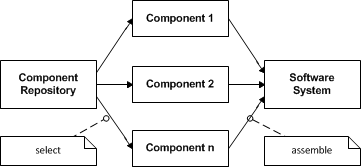
\includegraphics[scale=0.75]{plug-in/component-based.png}
  \caption{Component-based software development \cite{pour1998component} }
  \label{fig_cbsd}
\end{figure}

Other benefits that Component-based software development brings and we believe U-Sem will benefit from include: significant reduction of development cost and time-to-market, and also improvement on maintainability, reliability and overall qualities of software systems \cite{pour1999enterprise} \cite{pour1999making}. Additionally, the applicability of this approach is supported by the fact that it is widely used in both the research community and in the software industry. There are many examples of technologies implementing this approach including: OMG's CORBA \cite{vinoski1997corba},  Microsoft's Component Object Model (COM) and Distributed COM (DCOM) \cite{vinoski1997corba}, Sun's(now Oracle) JavaBeans and Enterprise JavaBeans \cite{goncalves2010enterprise}, OSGI \cite{tavares2008gentle}.


\subsubsection{Component model}

Designing the component model of a system provides the specification defining the way that the system can be build by composing different components applying the component-based software engineering approach. More formally, it is the architecture of a system or part of a system that is built by combining different components \cite{cai2000component}. It defines a set of  standards for component implementation, documentation and deployment. Usually, the main components that a component-based software system consists of are \cite{chen2009refinement}:

\paragraph{Interfaces}
	determine the external behaviour and features of the components and allow the components to be used as a black box. They provide the contract which defines the means of communication between components. As illustrated on figure \ref{fig_intf}, interfaces can be considered as points where custom functionality provided by another component can be plugged in. 
	
	\begin{figure}[h!]
  		\centering
  		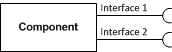
\includegraphics[scale=0.75]{plug-in/component-interfaces.png}
  		\caption{Component interfaces }
  		\label{fig_intf}
	\end{figure}

\paragraph{Components}
	are functional units providing functionality by implementing interfaces. As can be seen on figure \ref{fig_comp}, components provide  features by implementing the interfaces provided by other components. One of the main question regarding building components is how to define the scope and characteristics for a component. According to \cite{cai2000component} there are no clear and well established standards or guidelines that define this. In general, however, a component has three main features: 

\begin{itemize}
	\item a component is an independent and replaceable part of a system that fulfils a clear function
	\item a component works in the context of a well-defined architecture
	\item a component communicates with other components by its interfaces 
\end{itemize}

	\begin{figure}[h!]
  		\centering
  		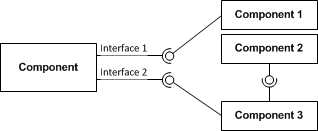
\includegraphics[scale=0.75]{plug-in/component-services.png}
  		\caption{Components implementing interfaces }
  		\label{fig_comp}
	\end{figure}

\paragraph{Coordinator}
	is the entity which is responsible to glue together and manage all the components. It is needed because components provide a number of features, but they are not able to activate the functionality themselves. This is the responsibility of the coordinator.

\subsubsection{State of the art component model implementations}

In previous sections, we discussed that integrating a component model in the architecture of U-Sem is the scientifically proven approach that promises to solve the design problem and fulfil the requirements of the customers. However, we had to decide whether to design and implement our own custom component model or we can reuse an existing one. Reusing a popular and widely used solution might be beneficial because it is likely it is heavily tested (at least from the engineers using it) and thus provide higher quality. 

\cite{lau2007software} suggests classification of the component model implementations based on which part of the life cycle of a system the composition of the components is done. They identify the following groups:

\begin{itemize}
	\item  Composition happens during the design phase of the system. Components are designed and implemented in the source code of the system.
	\item  Composition happens during the deployment phase. Components are constructed separately and are deployed together into the target execution environment in order to form the system.
	\item Composition happens during the runtime phase. Components are put together and executed in the running system.
\end{itemize}

For the architecture of U-Sem we are only interested in the last group since one of the main requirements is that engineers should be able to add, update and remove components while the system is running, without restarting it. This is essential since the system is used by multiple engineers and system restart will cause temporary unavailability of all services. 

Apart form this, there is also another critical concern when choosing component model implementation for U-Sem. The implementation should support the Java language since it is the language in which all current services are implemented and most engineers are familiar with. Having to learn a new language and/or rewriting all source code in different language is considered as a big disadvantage for the engineers.

We performed further investigation in order to find what are the current state of the art technologies that satisfy all requirements. It showed that currently there two standards that satisfy our needs: Fractal \cite{bruneton2006fractal} and Open Services Gateway initiative (OSGI) \footnote{OSGi Alliance. http://www.osgi.org}. Both of them seemed quite popular and widely used and therefore we concluded that reusing them is more beneficial than implementing a component model from scratch. For the proposed architecture of U-Sem we chose to use OSGI since our impression is that it provides a simpler way of defining components(no component hierarchies) which will be beneficial for engineers that do not have so in depth knowledge of component-based engineering. OSGI is also widely used \cite{tavares2008gentle} which may suggest that it is well tested and therefore is more stable. The next subsection focuses on how OSGI works and its features that are interesting for the architecture of U-Sem.


\subsubsection{OSGI}

Proposed first in 1998, OSGI represents a set of specifications that defines a component model which represents a dynamic component system for Java. These specifications enable a development model where applications are dynamically composed of different independent components. Components can be loaded, updated and deleted on demand without having to restart the system. OSGI defines the main components of the standard component model which are discussed in the previous section as follows:

\begin{figure}[h!]
  \centering
  	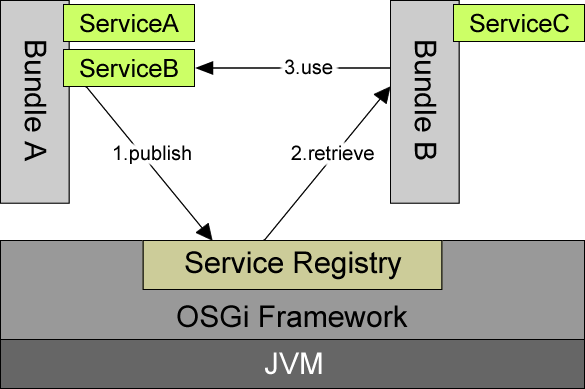
\includegraphics[scale=0.6]{plug-in/OSGI.png}
  \caption{OSGi Service Registry \cite{tavares2008gentle}}
  \label{fig_osgi}
\end{figure}

\paragraph{Interfaces}
 in OSGI define the contract for communication between different components by describing the operations that has to be implemented by the components. Basically, they represent standard Java interfaces or classes which has to be available to both the component that implements the interface and the components that use the implemented functionality.


\paragraph{Components}
  in OSGI are called bundles. Bundles are basically a regular Java JAR files that contain class files and other resources such as images, icons, required libraries. One of the important benefits for U-Sem is that OSGI enables better modularization providing facilities for better information hiding then the one provided by the Java language \cite{tavares2008gentle}. Each bundle should provide a manifest file, which enables engineers to declare static information about the packages that are exported and therefore can be used by other bundles. Furthermore, bundles provide functionality to the rest of the system in the form of services. In the OSGi architecture, services are standard Java objects that implement the interfaces described in the previous paragraph.

\paragraph{Coordinator}
The OSGi standard also provides coordinator component which represents a runtime infrastructure for controlling the life cycle of the bundles which includes adding, removing and replacing bundles at run-time, while preserving the relations and dependencies among them. Another key functionality that the coordinator component of OSGi provides is the management of the services provided by the bundles. This functionality is provided by the Service Registry, which keeps track of the services registered within the framework. As illustrated on Figure \ref{fig_osgi}, when a bundle is loaded it registers all the services that it implements(step 1). As soon as a service is registered, it can be retrieved by any other components that are interested in this functionality (step 2). Once a bundle has retrieved a service, it can invoke any method described by the interface of this service (step 3). Another interesting feature of the OSGi Service Registry is its dynamic nature. As soon as a one bundle publishes a service that another bundle is interested in, the registry will bind these two bundles. This feature is very important for U-Sem since it will enable engineers to plug in any new functionality dynamically when it is needed.

\subsubsection{Security}

The security capabilities of OSGI are also very important for U-Sem since a lot of custom code is being executed which poses a significant threat to the system. The OSGi platform is considered to be highly secure by its creators \cite{parrend2009security}. There are two main reasons in favour of this statement. Firstly, OSGi is executed on top of the JVM and inherits its security capabilities. Secondly, it has been designed to support a proper level of isolation between components.

Since its introduction, the Java language and JVM have been widely used and subjected to extensive tests and validation \cite{parrend2009security}. The platform was designed to support the safe execution of fully untrusted code \cite{dean1996java}. In order to achieve this, it has introduced the following features \cite{gong2003inside}: Type Safety of the language, Garbage Collection(no user-defined memory management), Bytecode verification ensuring that executed programs are compliant with the language specification, and Sandboxing, which can prevent the access to sensible resources like the network or file system. Additionally, the system provides secure class loaders, which enable loading of several modules that cannot interact with each other.

On top of this, OSGI defines additional permissions that provides full control of the interactions between the components. It provides functionality that enables dependencies at the package level and at the service level to be allowed or prevented. Additionally, management capability from one component to the others can also be restricted \cite{parrend2009security}.

\subsection{Collaboration between users}

Engineers have to be able to collaborate between each other by reusing each others functionality. In order to support this feature we propose an approach based on the \textit{Component Repository} idea \cite{seacord1999software}. We introduce a plug-in repository which represents a storage location where plug-ins are stored and when needed, they can be retrieved and installed into the system. When engineers build a new plug-in then they can share it with other scientist by publishing it at the repository so that anyone interested can install and use it. The applicability of this approach is also supported by the fact it is used in other plug-in based systems like Eclipse \cite{mcaffer2010eclipse} as well.

Using the plug-in repository engineers are able to exchange components before they are installed into U-Sem. Alternative approach would have been enable engineers to share already installed components between each other. In this way, whenever an engineer creates a new version or an entirely new component it is installed to U-Sem, shared and then all other engineers are able to use it. However, that approach has one major disadvantage. When a new version of a component is installed then all engineers automatically start to use the new version. The version, though, might introduce a bug or it might not be completely compatible with the previous version. As a result, all other engineers' services and components that are using it are threatened to experience failures. 

Using the Plug-in repository overcomes this problem. When a engineer releases new version of component, other engineers can decide whether or not to immediately adopt the new release. If they decide not to, they can simply continue using the old one. 
Later, when they decide that are ready for the change, they install and use the new release. The benefit from this approach is that none of the engineers are at the mercy of the others. Changes made to one component do not need to have an immediate affect on other engineers that are using it. Each engineer can decide whether or when to move to the new releases of the components in use.

\subsection{Dependencies management}

It is very likely that plug-ins have dependencies between each other. This may be as a result of reusing functionality from other engineer's plug-ins or depending on a plug-in that provides common functionality like extracting data from social media and storing data into a database. In order to use such plug-in engineers have to make sure that all its dependent plug-ins are also installed. The problem is that the dependency information is only available on compile time. Once the plug-in is compiled it hard to tell what are its dependencies because this information is packed inside the \textit{Jar} file representing the plug-in. Therefore, engineers are responsible to remember what are the dependencies of the plug-ins they are installing or to refer to the source code. This problem is even more severe when engineers reuse shared plug-ins from the plug-in repository since they do not have access to their source code and therefore, have to contact and communicate the dependencies with the owners of the plug-ins which is an obvious overhead and waste of time. We believe that this approach for dealing with the plug-in dependencies is not effective and will pose a significant overhead for engineers.

Literature suggests that there is an already existing attempt to overcome this problem which is the Eclipse P2 framework \cite{le2009dependency}. It represents a component provisioning system that can be configured to work with any kind of components (not only plug-ins) and proposes the idea of packing components into installable units that define the dependencies between them. Clients of the system install the entire installable units which ensures that all the required components will be installed. The framework, however, is designed to be flexible in order to be applicable for a variety of different scenarios and as a result requires a lot of additional work from the engineers in order to set all the installable units up which is a big disadvantage for the U-Sem scenario. Therefore, we propose a simpler approach specifically designed for solving the problem in U-Sem. It is based on the fact that U-Sem is designed to work only with OSGi plug-ins which already contain information about the dependencies. As a result, the system can automatically read these dependencies and verify if they are all satisfied and the system is consistent. The proposed solution consists of two parts:

\begin{itemize}
	\item The Plug-in repository is extended so that when a new plug-in is being installed it checks the current configuration and any missing dependent plug-ins are offered for installation as well.
	\item The system is also extended so that it looks for and notifies the engineers in case of any missing dependencies. It  proposes their installation from the plug-in repository if they are present there.
\end{itemize}


The main benefit from this approach is that it completely automates the dependency management process and does not require any additional work from the engineers when they are building plug-ins. There is, however, one use-case which requires some manual work. It originates from the fact that in certain cases OSGI also allows plug-ins to depend on Java packages without specifying their source \cite{bartlett2009osgi}. This is not a significant problem for U-Sem since this functionality is only used for plug-ins to refer to the packages which are not encapsulated in plug-ins like the workflow engine. This packages are already part of the plug-in environment and therefore, no action is required. If there is still a future use-case where this "indirect" dependencies are needed engineers are responsible to manage them manually.


\subsection{Plug-in construction support}

In order to create a plug-in engineers have to create and configure a plug-in project. This process involves setting up all required dependencies and building the required folder structure within the project. From engineers' point of view, all these steps are considered as an overhead that can be time consuming especially for new members of the team or for engineers without computer science background. Therefore, in order to automate this process the system provides a special Eclipse based SDK (software development kit) which extends the out-of-the-box capabilities of Eclipse providing user interface that assists engineers to easily create and set-up plug-ins for U-Sem. This is achieved by introducing a special \textit{Eclipse Project Template} \cite{silva2009practical} that can automatically create U-Sem plug-ins, set up their folder structure and add the required dependencies. Additionally, often engineers have to create simple one-component workflows in order to test a specific component. The solution is also capable automate this process by allowing engineers to create plug-in projects with pre-wired one-component workflows. Engineers only have to provide the names of the component and the workflow in the user interface and put the source code into the Java class dedicated for the created component. 

Having identified an approach for solving each of the issues concerning the Plug-in Environment feature we continue by discussing the architecture and implementation of the solution covered in the next sections. 

\section{Architecture}
\label{sec:architecturePlugin}

Based on the approach devised in the previous section we designed the software architecture for the \textit{Plugin Environment} feature of U-Sem. In this section we provide the description of the proposed architecture focusing on the static and dynamic structures of the solution and its externally visible behaviour.

One of the critical things when describing a software architecture is to manage complexity of the description so that it is clear and understandable by the stakeholders. \cite{rozanski2011software} suggests that capturing the essence and all details of the whole architecture in a single model is only possible for very simple systems. Doing this for a more complex system is likely to end up as a model that is unmanageable and does not adequately represent the system to you or any of the stakeholders. \cite{rozanski2011software} also claims that the best way to deal with the complexity of the architecture description is to break it into a number of different representations of all or part of the architecture, each of which focuses on certain aspects of the system, showing how it addresses some of the stakeholder concerns. These representations are called views.

In next sections, we provide a set of interrelated views, which collectively illustrate the functional and non-functional features of the system from different perspectives and demonstrate that it meets the requirements. Note that in the reminder of this chapter we use the term \textit{plug-in} for the components containing the custom functionality provided by engineers. In this way they are easily distinguished from the architectural components. 

\subsection{Context View}

The Context view aims to define the environment in which the system operates and more specifically the technical relationships that the system has with the various elements of this environment \cite{woods2009system}. \cite{woods2009system} also identifies the concerns that the view has to address:

\begin{itemize}
	\item Identify which are the external entities and what are the responsibilities of each of them.
	\item Identify the dependencies between the external entities which affect the system.
	\item Identify the the nature of the connections between the entities.
	\item Define the interactions that are expected to occur over the connections between the entities.
	\item Define what are the system's external interfaces.
\end{itemize}


As explained in the introduction section, initially, the system only communicated with providers of semantic content and the clients which execute the services defined by the engineers. The way the interactions work is not affected by the architecture discussed in this chapter. Introducing the Plug-in Environment feature, however, brings two new entities on the stage: engineers providing user modelling components for U-Sem and a Plug-in repository supporting the collaboration between engineers. Figure \ref{fig_context} illustrates the updated runtime environment of U-Sem.


\paragraph{Engineers}
In order to be able to construct user modelling workflows, engineers first have to build and deploy the required components that are needed for the workflows. In order to do that, engineers first have to build a plug-in that encapsulates the new functionality defining the components. Then, they upload the plug-in to U-Sem through a web user interface and it will be installed in the storage space of the engineer. Once installed, the engineer can start using the newly added functionality. Additionally, engineers can also communicate with U-Sem in order to manage the existing plug-ins loaded into the system. Using a web user interface, they can view the list of all available components and if needed they can even remove some of them.

\begin{figure}[h!]
  \centering
  	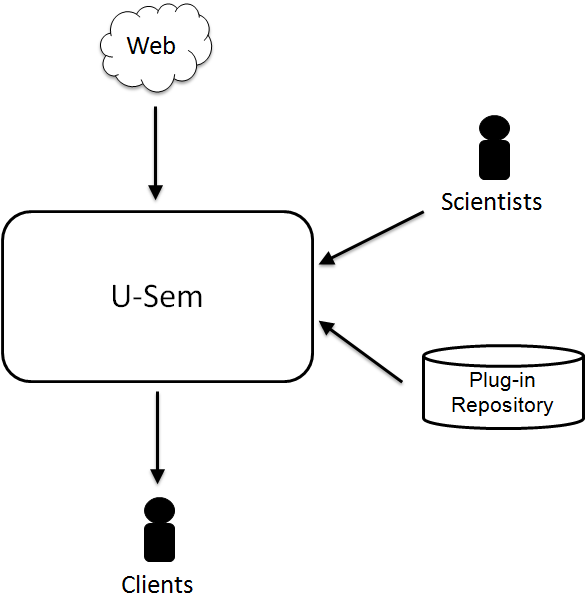
\includegraphics[scale=0.5]{plug-in/environment/runtime_env.png}
  \caption{Context diagram of U-Sem }
  \label{fig_context}
\end{figure}

\paragraph{Plug-in repository}
It represents a storage location where plug-ins are stored and when needed, they can be retrieved and installed into the system. engineers build and then publish their plug-ins there so that anyone interested can install and use them. 


\subsection{Interactions}

After we have identified the new actors(engineers) and external systems(plug-in repository) in the environment of U-Sem we have to define how they interact with each other. In this section we use the Business Process Management Notation(BPMN) \cite{wohed2006suitability} to define the business processes that describe the interactions needed for each of the use cases regarding the dynamic component model feature of U-Sem. The notation enables us to model activities, decision responsibilities, control and data flows. The decision to use BPMN to define the interactions is based on its suitability for interaction modelling and the fact that it is more popular compared to its alternatives \cite{decker2008interaction}. Next subsections describe each of the defined processes and expand them into Business Process Diagrams (BPD).

\subsubsection{Create U-Sem Plug-in process}

\begin{figure}[h!]
  \centering
  	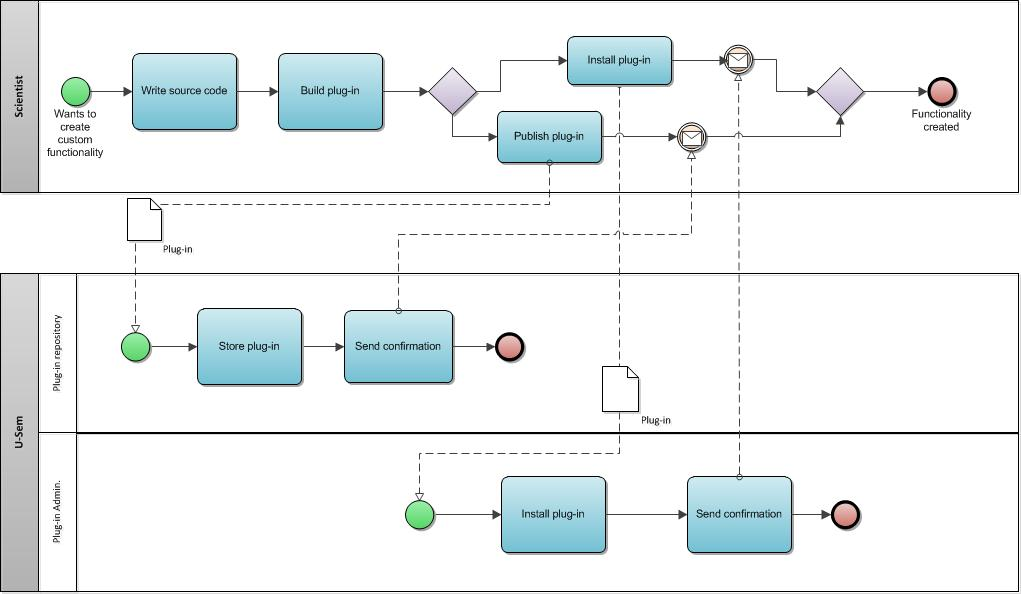
\includegraphics[scale=0.7,angle=270]{plug-in/business_processes/CreatePlugInBusinessModel.jpg}
  \caption{Business model describing the process for creating a new plug-in for U-Sem}
  \label{fig_install_bpm}
\end{figure}

In this section, we modelled the plug-in creation process as a business process. Figure \ref{fig_install_bpm} provides the business process model diagram that illustrates this process. 

As illustrated in the diagram, there are three participants in this process(U-Sem, engineers and the Plug-in repository) which are illustrated in separate BPMN pools. When a engineer wants to create new functionality for U-Sem, he/she first writes the source code, providing all required resources and implementing the desired U-Sem interfaces(the component interfaces discussed in previous sections). Then, everything is built and encapsulated into a single plug-in. If it is only for private use, engineers can directly upload it to U-Sem . When U-Sem receives a component it is responsible to install it into the engineer's dedicated storage space and make available all functionality provided by the component. Finally, U-Sem sends confirmation message back to the engineer. Alternatively, the engineer might also want to share the component with other engineers. In this case, the component is sent to the plug-in repository. When received, the repository is responsible to store it and make it available to the other engineers. Again, at the end a confirmation message is sent back to the engineer.

\subsubsection{Reuse shared plug-ins}

\begin{figure}[h!]
  \centering
  	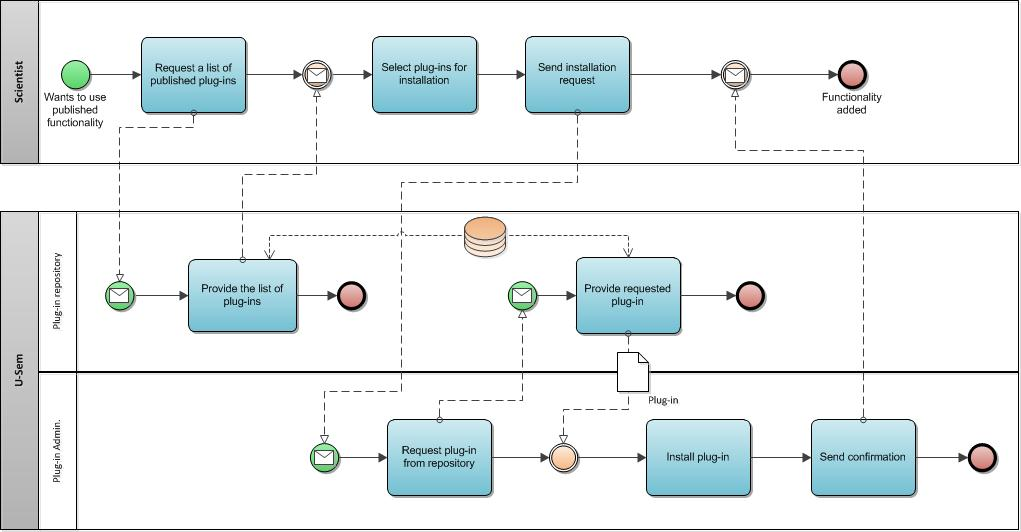
\includegraphics[scale=0.7,angle=270]{plug-in/business_processes/InstallPlugInFromRepoBusinessModel.jpg}
  \caption{Business model describing the process for installing a shared plug-in/s to U-Sem}
  \label{fig_repo_bpm}
\end{figure}

As defined in section \ref{sec:requirementsPlugin}, U-Sem also enables engineers to reuse plug-ins shared by others. This use case is also modelled as a separate business process which is illustrated in Figure \ref{fig_repo_bpm}. Again, we have three participants in this process(U-Sem, engineers and the Plug-in repository) which are illustrated in separate BPMN pools. 

The process consists of two main phases. First, the engineer contacts the plug-in repository in order to determine what are the currently available plug-ins and then, he/she contacts U-Sem providing information about the desired plug-ins. Upon receiving the request, U-Sem is responsible to contact the plug-in repository and retrieve the requested plug-ins which are, at the end, installed into the private space of the engineer and a confirmation message is send back.

\subsubsection{Plug-in Management}

\begin{figure}[h!]
  \centering
  	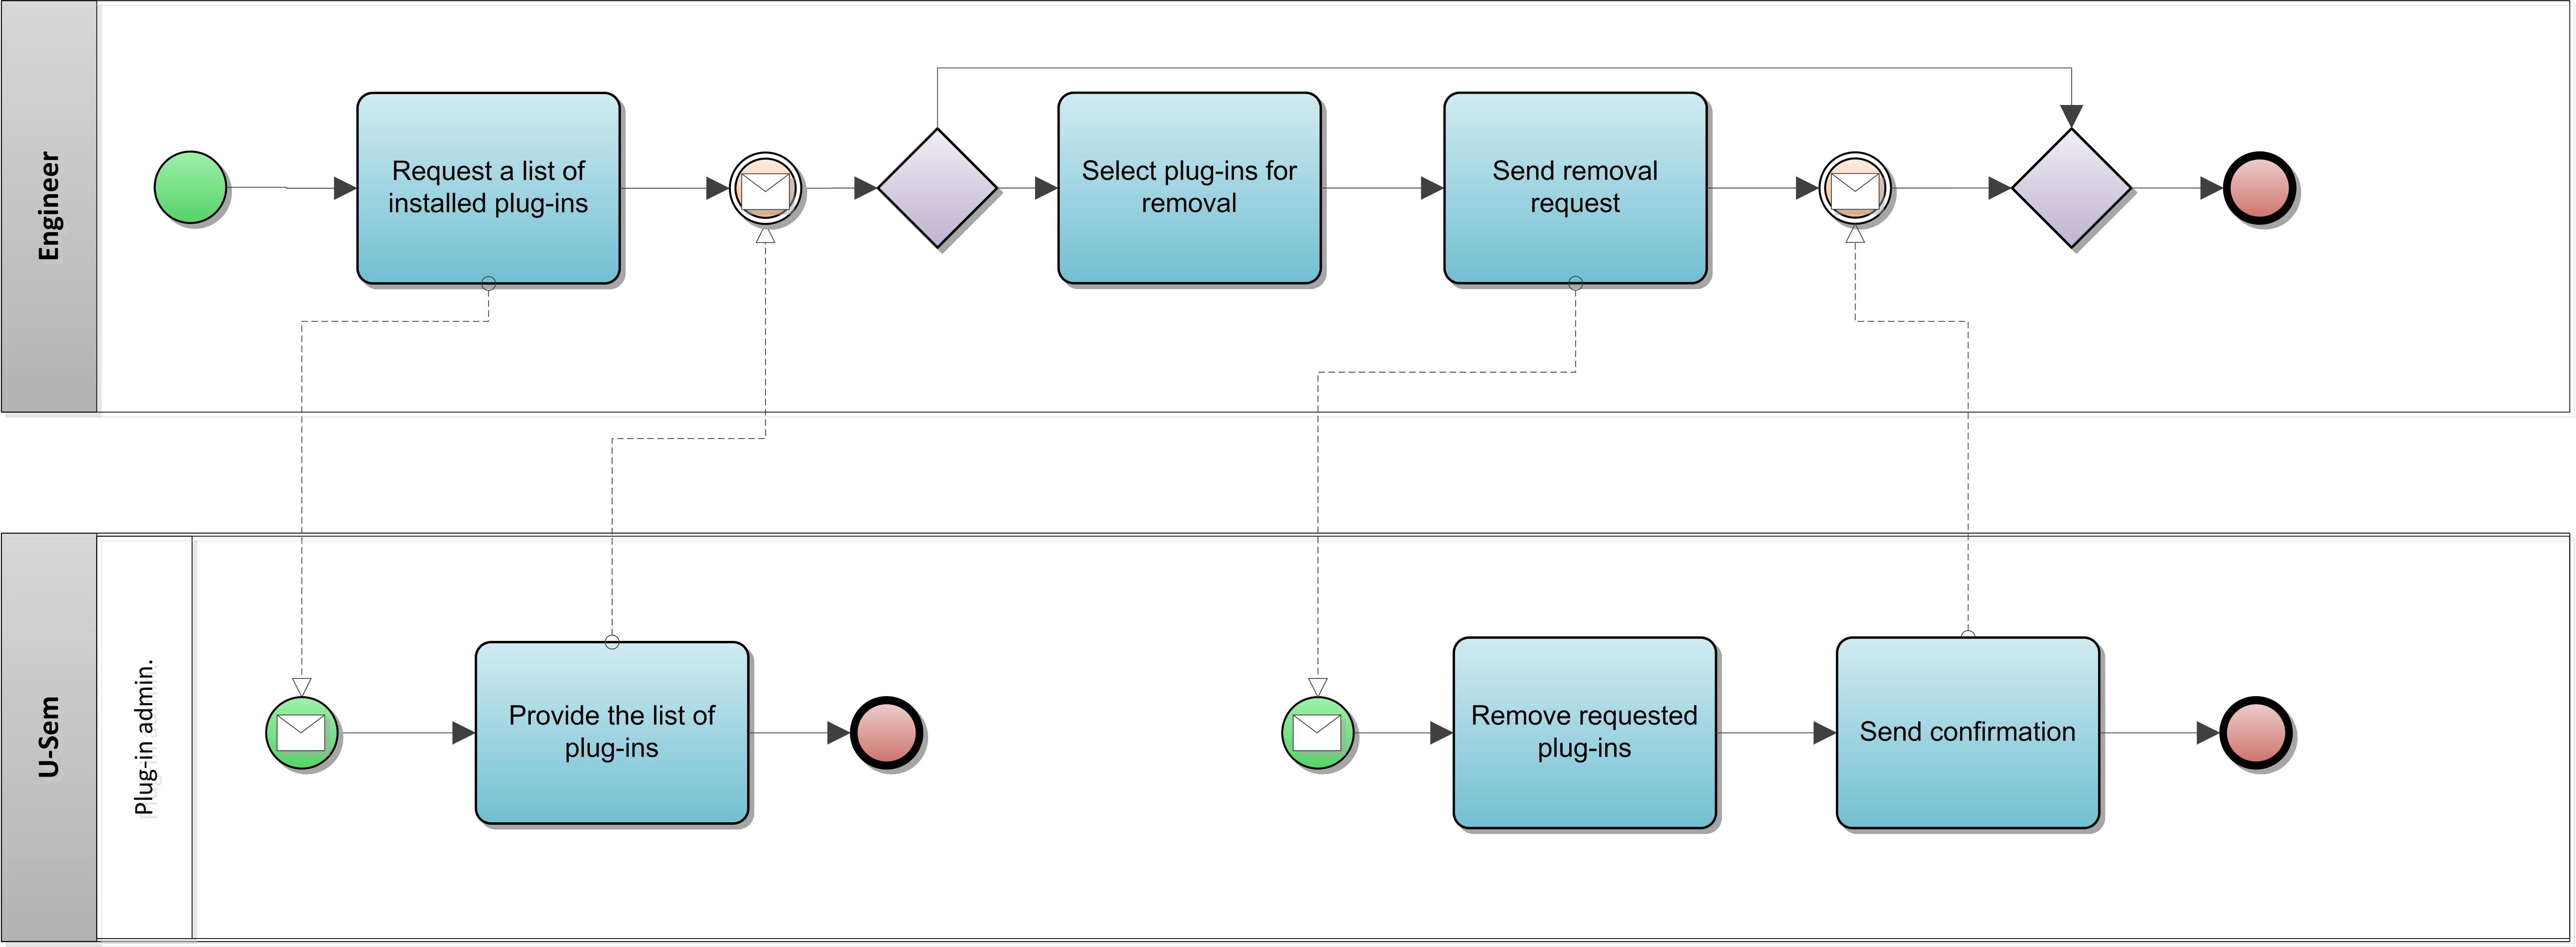
\includegraphics[scale=0.7,angle=270]{plug-in/business_processes/PluginManagementBusinessModel.jpg}
  \caption{Business model describing the process for managing plug-ins in U-Sem}
  \label{fig_admin_bpm}
\end{figure}

Managing plug-ins is also another important use case. Implementing it enables engineers to view all plug-ins installed into U-Sem and if needed remove any of them. This use case was modelled into the \textit{Plug-in Management process} which is illustrated on Fugure \ref{fig_admin_bpm}. In this case, we have interaction only between the engineer and U-Sem.

engineers can monitor the currently installed plug-ins at any time by contacting U-Sem. When such request is received, U-Sem is responsible to send back detailed information about all the plug-ins. Having this list, engineer are also able to remove plug-ins. In this case, engineers have to submit request for removal providing details for the plug-in that has to be removed. Upon receiving a request for plug-in removal, U-Sem is responsible to permanently remove it form the private space of the engineers and when finished send back a confirmation message.


\subsection{Functional view}

After identifying all actors that are part of the environment of U-Sem and the way they interact with one another, in this section, we define the internal structure of U-Sem that is responsible to accommodate all these interactions. The functional structure of the system includes the key functional elements, their responsibilities, the interfaces they expose, and the interactions between them \cite{rozanski2011software}. All these together demonstrate how the system will perform the required functions.

All components that take part in the dynamic component model functionality can be classified in three layers. This organization is illustrated in figure Figure \ref{fig_layer} and consists of the following layers:

\begin{figure}[h!]
  \centering
  	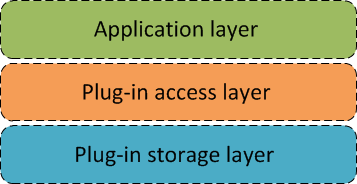
\includegraphics[scale=0.6]{plug-in/layers/layers.png}
  \caption{Layered organization of the solution}
  \label{fig_layer}
\end{figure}

\begin{itemize}
	\item \textit{Plug-in storage layer} is responsible to provide storage functionality for storing the installed plug-ins. Additionally, it should provide place where plug-ins can store data during their execution.
	\item \textit{Plug-in access layer} provides functionality for plug-in management and provides access to services provided by the plug-ins. The functional components that build this layer are responsible to enforce the security and privacy policies of the system.
	\item \textit{Application layer} this layer consists of all functional components that are interested in using the services provided by the plug-ins. These applications are also responsible to provide functionality to the user for adding new plug-ins to the system or managing the existing ones. 
	\end{itemize}

\subsubsection{High-level component organization}

This section describes the internal structure of the layers and identifies the high level components that build up the feature. Figure \ref{fig_comp} illustrates this organization. It shows how the high-level components are organized into the layers and the way they depend on each other. We have identified the following high level components:

\begin{figure}[h!]
  \centering
  	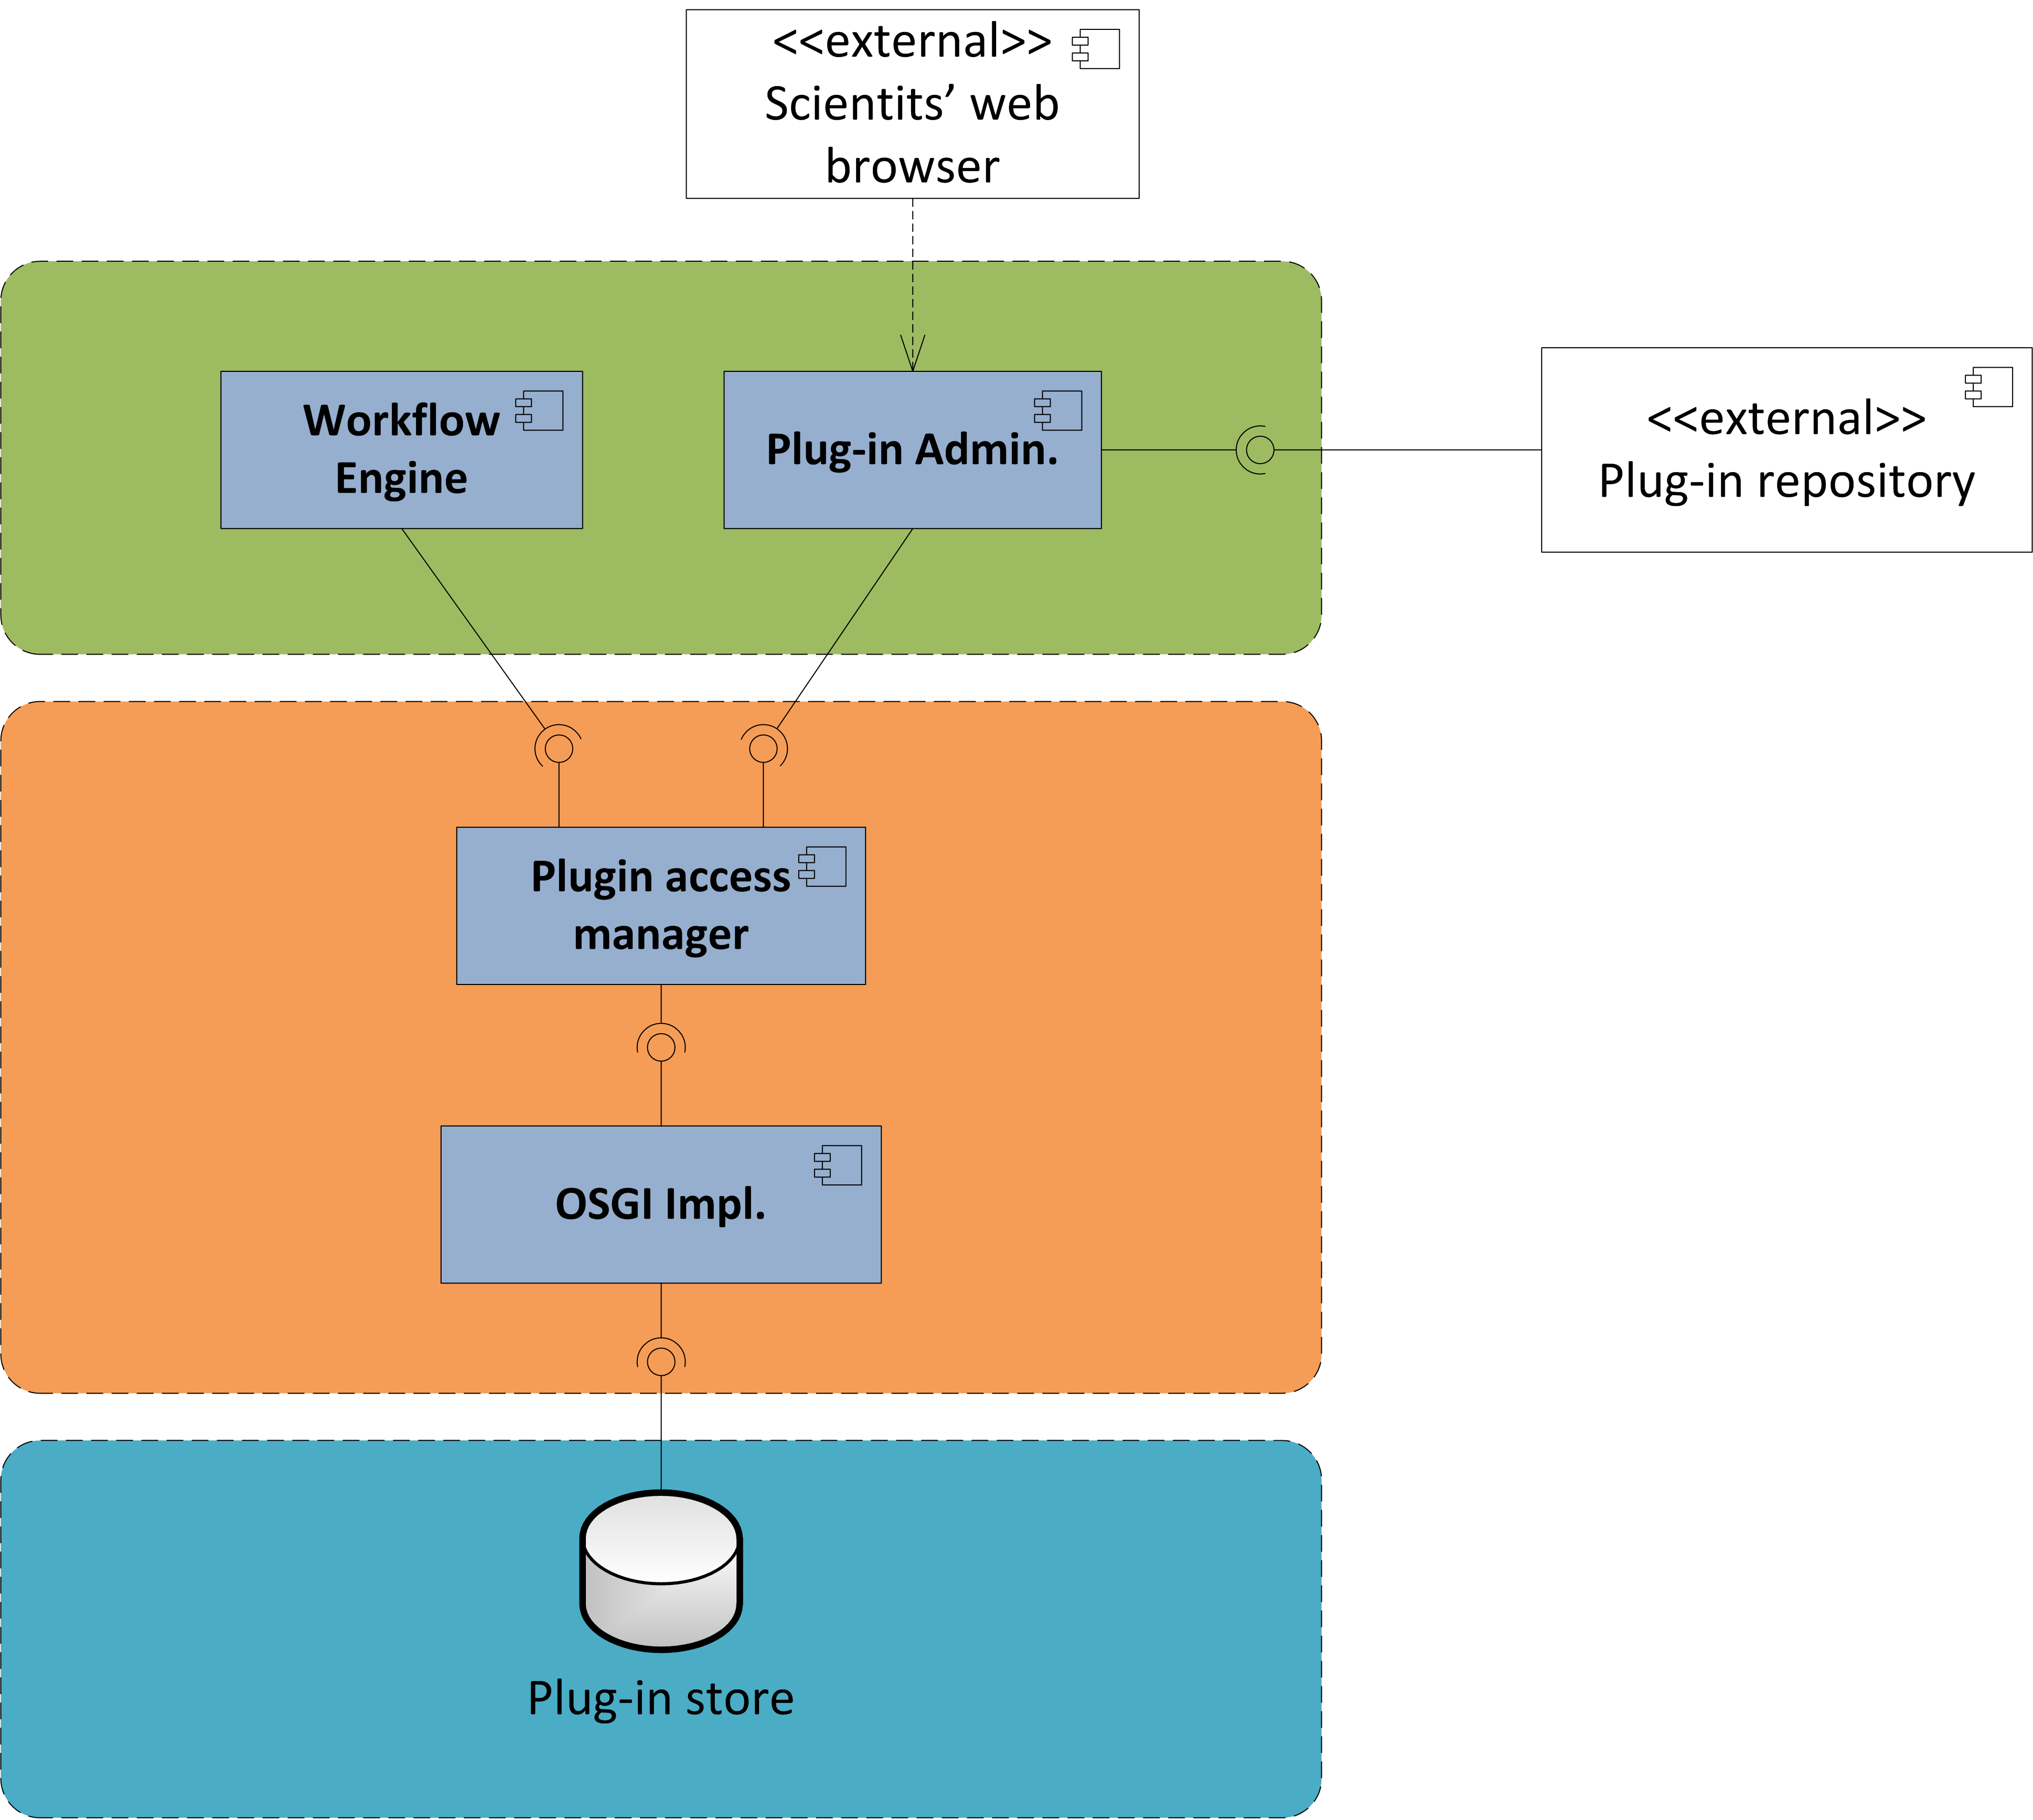
\includegraphics[scale=0.6]{plug-in/layers/main-func.png}
  \caption{Component diagram illustrating the functional organization of the solution}
  \label{fig_comp}
\end{figure}

\begin{itemize}

\item \textit{Plug-in Store} is responsible to store the installed plug-ins for each user. It should provide permanent store for the components so that after system restart they are still available. This component is also responsible to provide storage space for each component in case any data storage is required. It has to ensure that at any point of time the data is secured and backed up. The current state of OSGI only allows integration with file systems for plug-in storage and therefore, this component has to provide file system interface for communication.

\item \textit{OSGI Implementation} - As we already discussed in previous sections, we will use the OSGI standard as a base for providing the dynamic component model for U-Sem. It is responsible to mange the plug-ins' life cycle and provide access to the services implemented by the different components. It provides an API which enables other components to communicate with the framework.

\item \textit{Plug-in access manager} acts as a level of abstraction over the OSGI component. It is responsible to deal with the configuration and manage the life cycle of the OSGI framework. It is also responsible to enforce the security policy and provide isolation between engineers. It provides API for the application layer components for dealing with services and management of plug-ins. Further decomposition of this component is provided in the next sections.

\item \textit{Plug-in admin} is responsible to deal with the administration of the plug-ins. It provides the system's endpoint(user interface) for interaction with the engineers. Additionally, it also provides functionality for communication with the plug-in repository. Further decomposition of this component is provided in the next section. 

\item \textit{Workflow engine} uses the interface provided by the \textit{Plug-in access manager} to access the services implemented by the components. During the workflow configuration phase it uses the interface in order to obtain the list of available services implemented by the components, while during the workflow execution phase it uses the interface to execute and retrieve the result of the services.
	
\end{itemize}


\subsubsection{Plug-in admin}

This section defines the functional decomposition of the \textit{Plug-in admin} component which is illustrated on figure \ref{fig_admin_func}. It consists of the following components:

\begin{figure}[h!]
  \centering
  	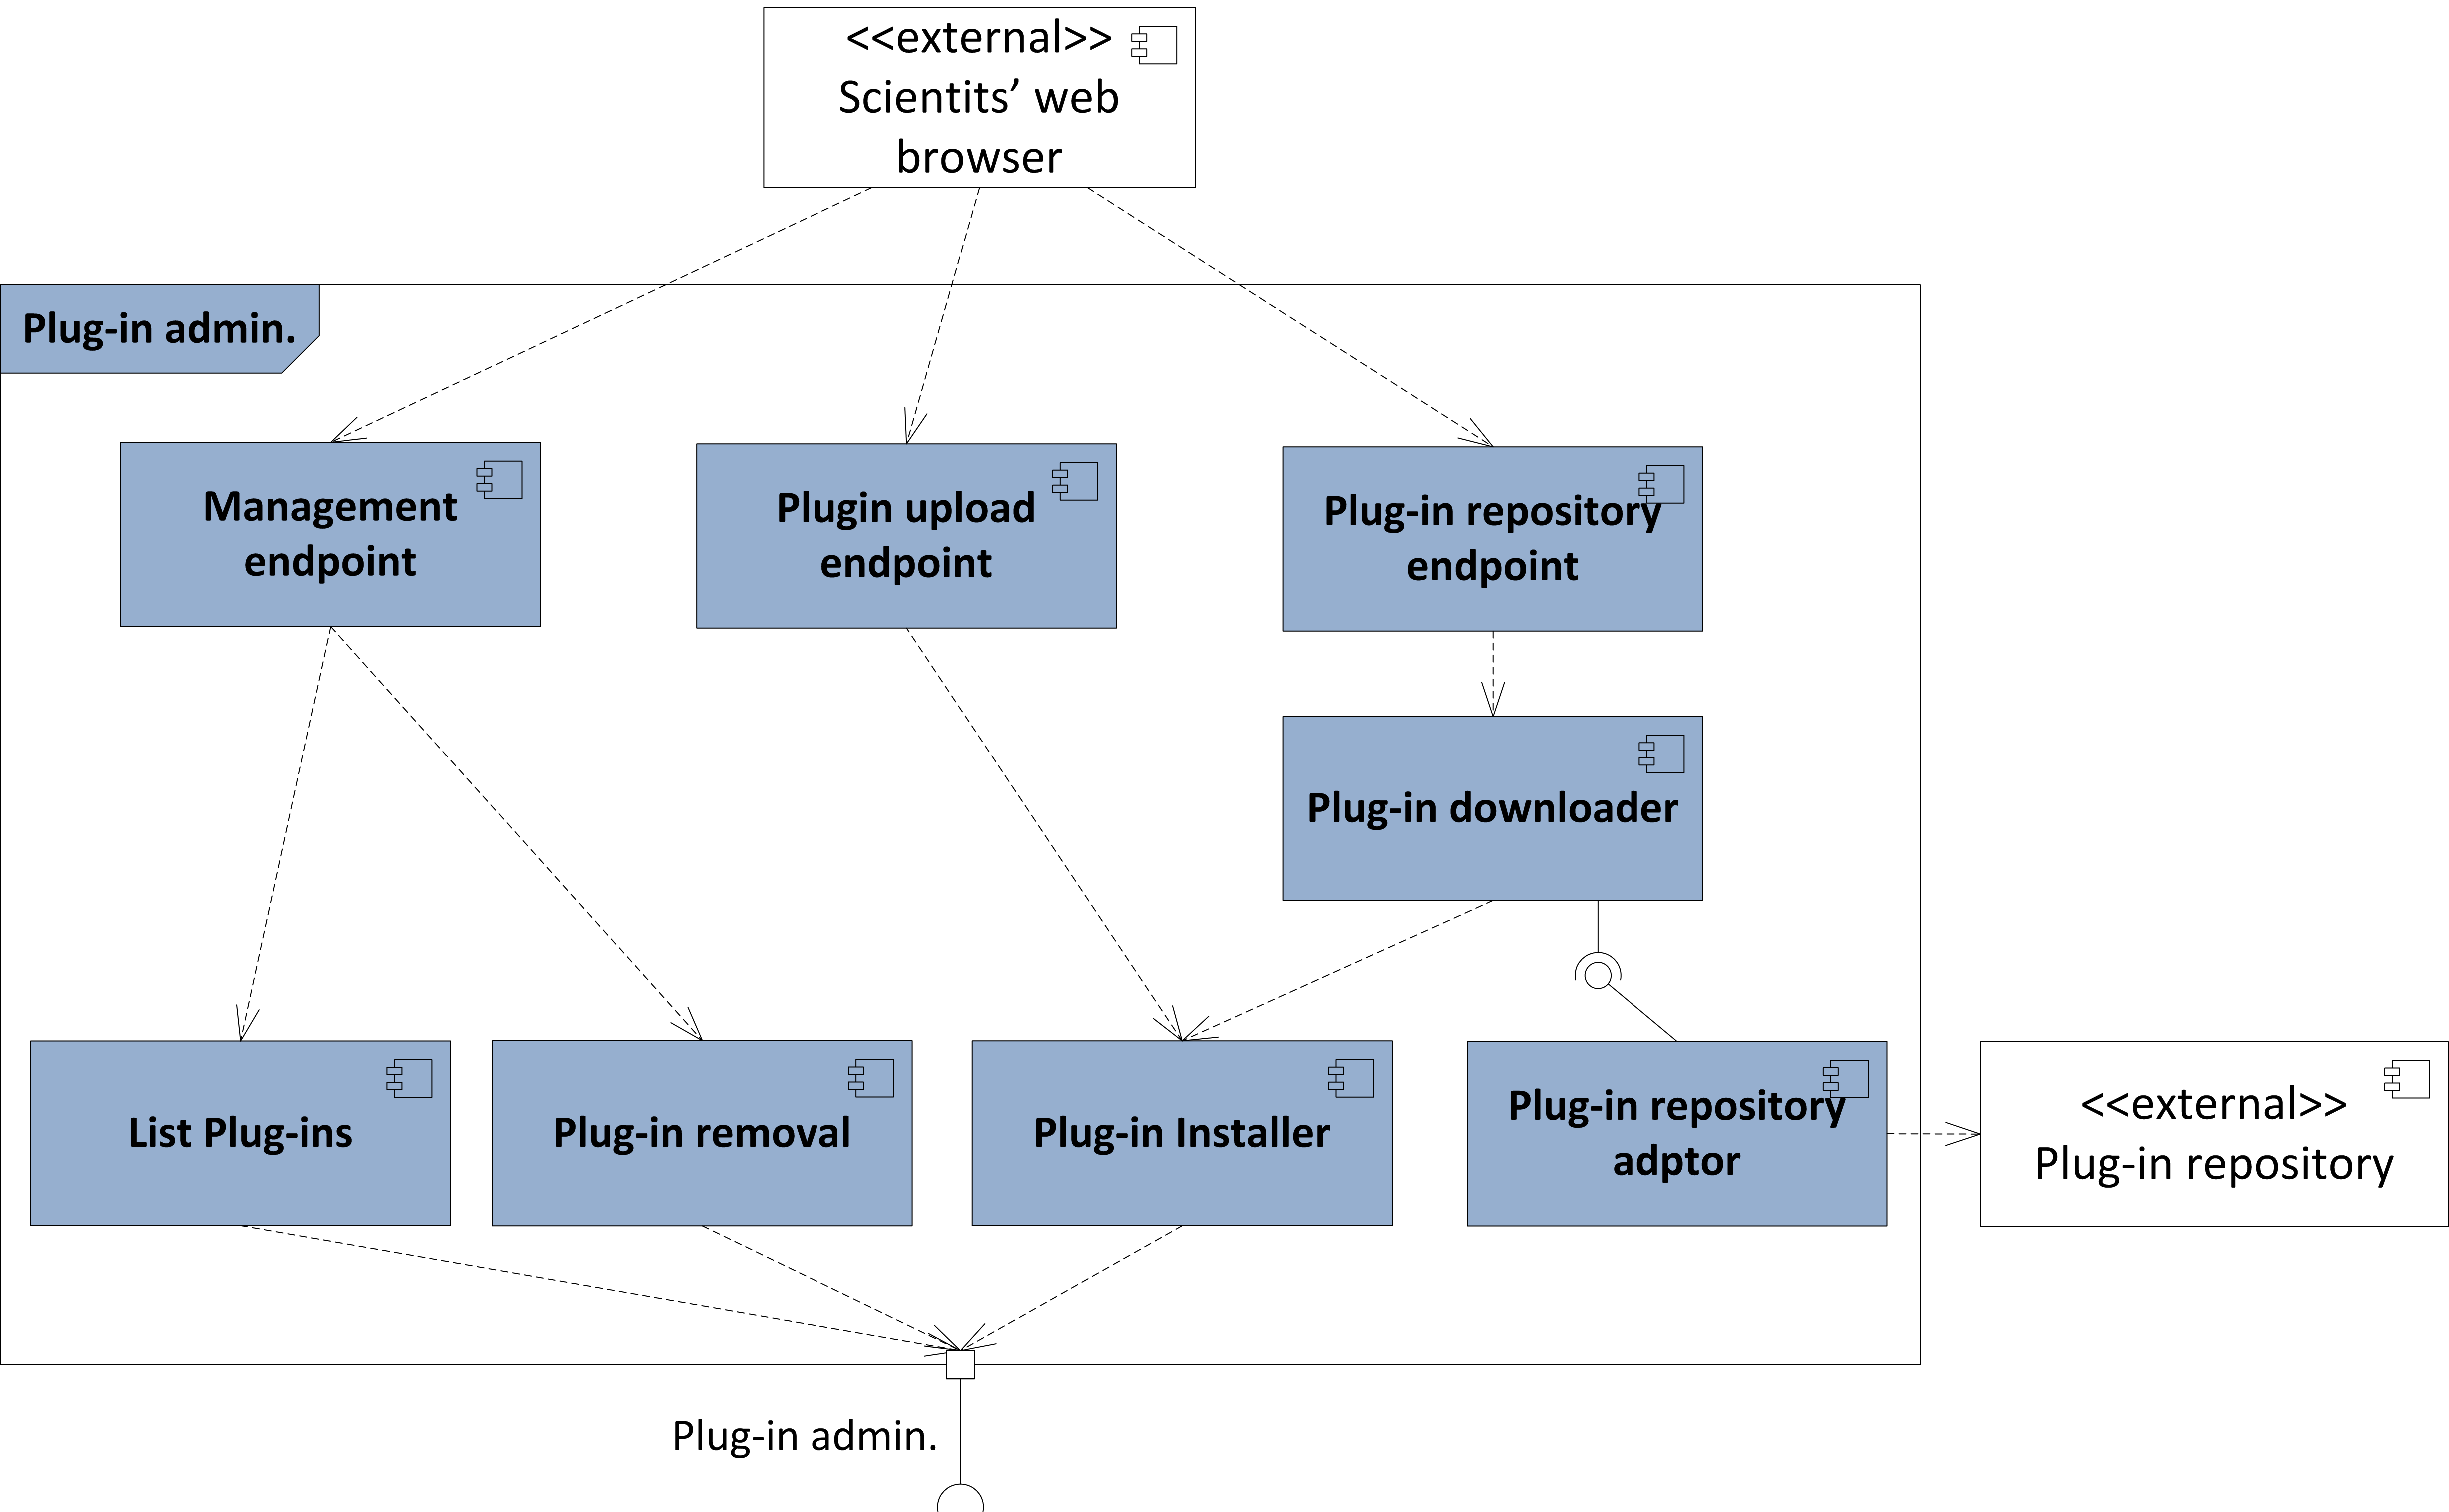
\includegraphics[scale=0.75]{plug-in/layers/admin-func.png}
  \caption{Functional decomposition of the \textit{Plug-in admin.} module}
  \label{fig_admin_func}
\end{figure}

\begin{itemize}

\item \textit{Management endpoint} - This component provides the user interface for the plug-in management functionality. It acts as a bridge between the user and the Plug-in admin. API. It uses the API in order to present the current state of the system to the users and also enable them to remove any components. This component also checks the dependencies between the installed plug-ins and notifies the user if any of them are missing.

\item \textit{Plug-in upload endpoint} - This components provides the user interface needed for uploading plug-ins. It enables users to select a \textit{jar} file from their local file system and upload it for installation. When the plug-in is uploaded to U-Sem it is installed using the Plug-in admin. API.

\item \textit{Plug-in repository endpoint} - This component provides the user interface which enables users to browse the plug-in repository and indicate which plug-ins should be downloaded and installed on U-Sem. It checks the dependencies of the selected plug-ins and if any are missing it notifies the user and proposes to install the missing plug-ins as well. Finally, the selected plug-ins are downloaded from the repository and upon successful download they are installed using the Plug-in admin. API.

\item \textit{Plug-in repository adaptor} - This component manages  the communication with the plug-in repository. It acts as a level of abstraction over it. U-Sem might evolve in future and need to use different repositories and in that case, this is the only component to change if support for a new repository system is needed. 

\end{itemize}


\subsubsection{Plug-in access manager}

This component is responsible to provide API which can be used by application layer components in order to manage the plug-ins and access the functionality provided by them. Figure \ref{fig_access_func} shows the functional decomposition of the Plug-in access manager module. It consists of the following components:


\begin{figure}[h!]
  \centering
  	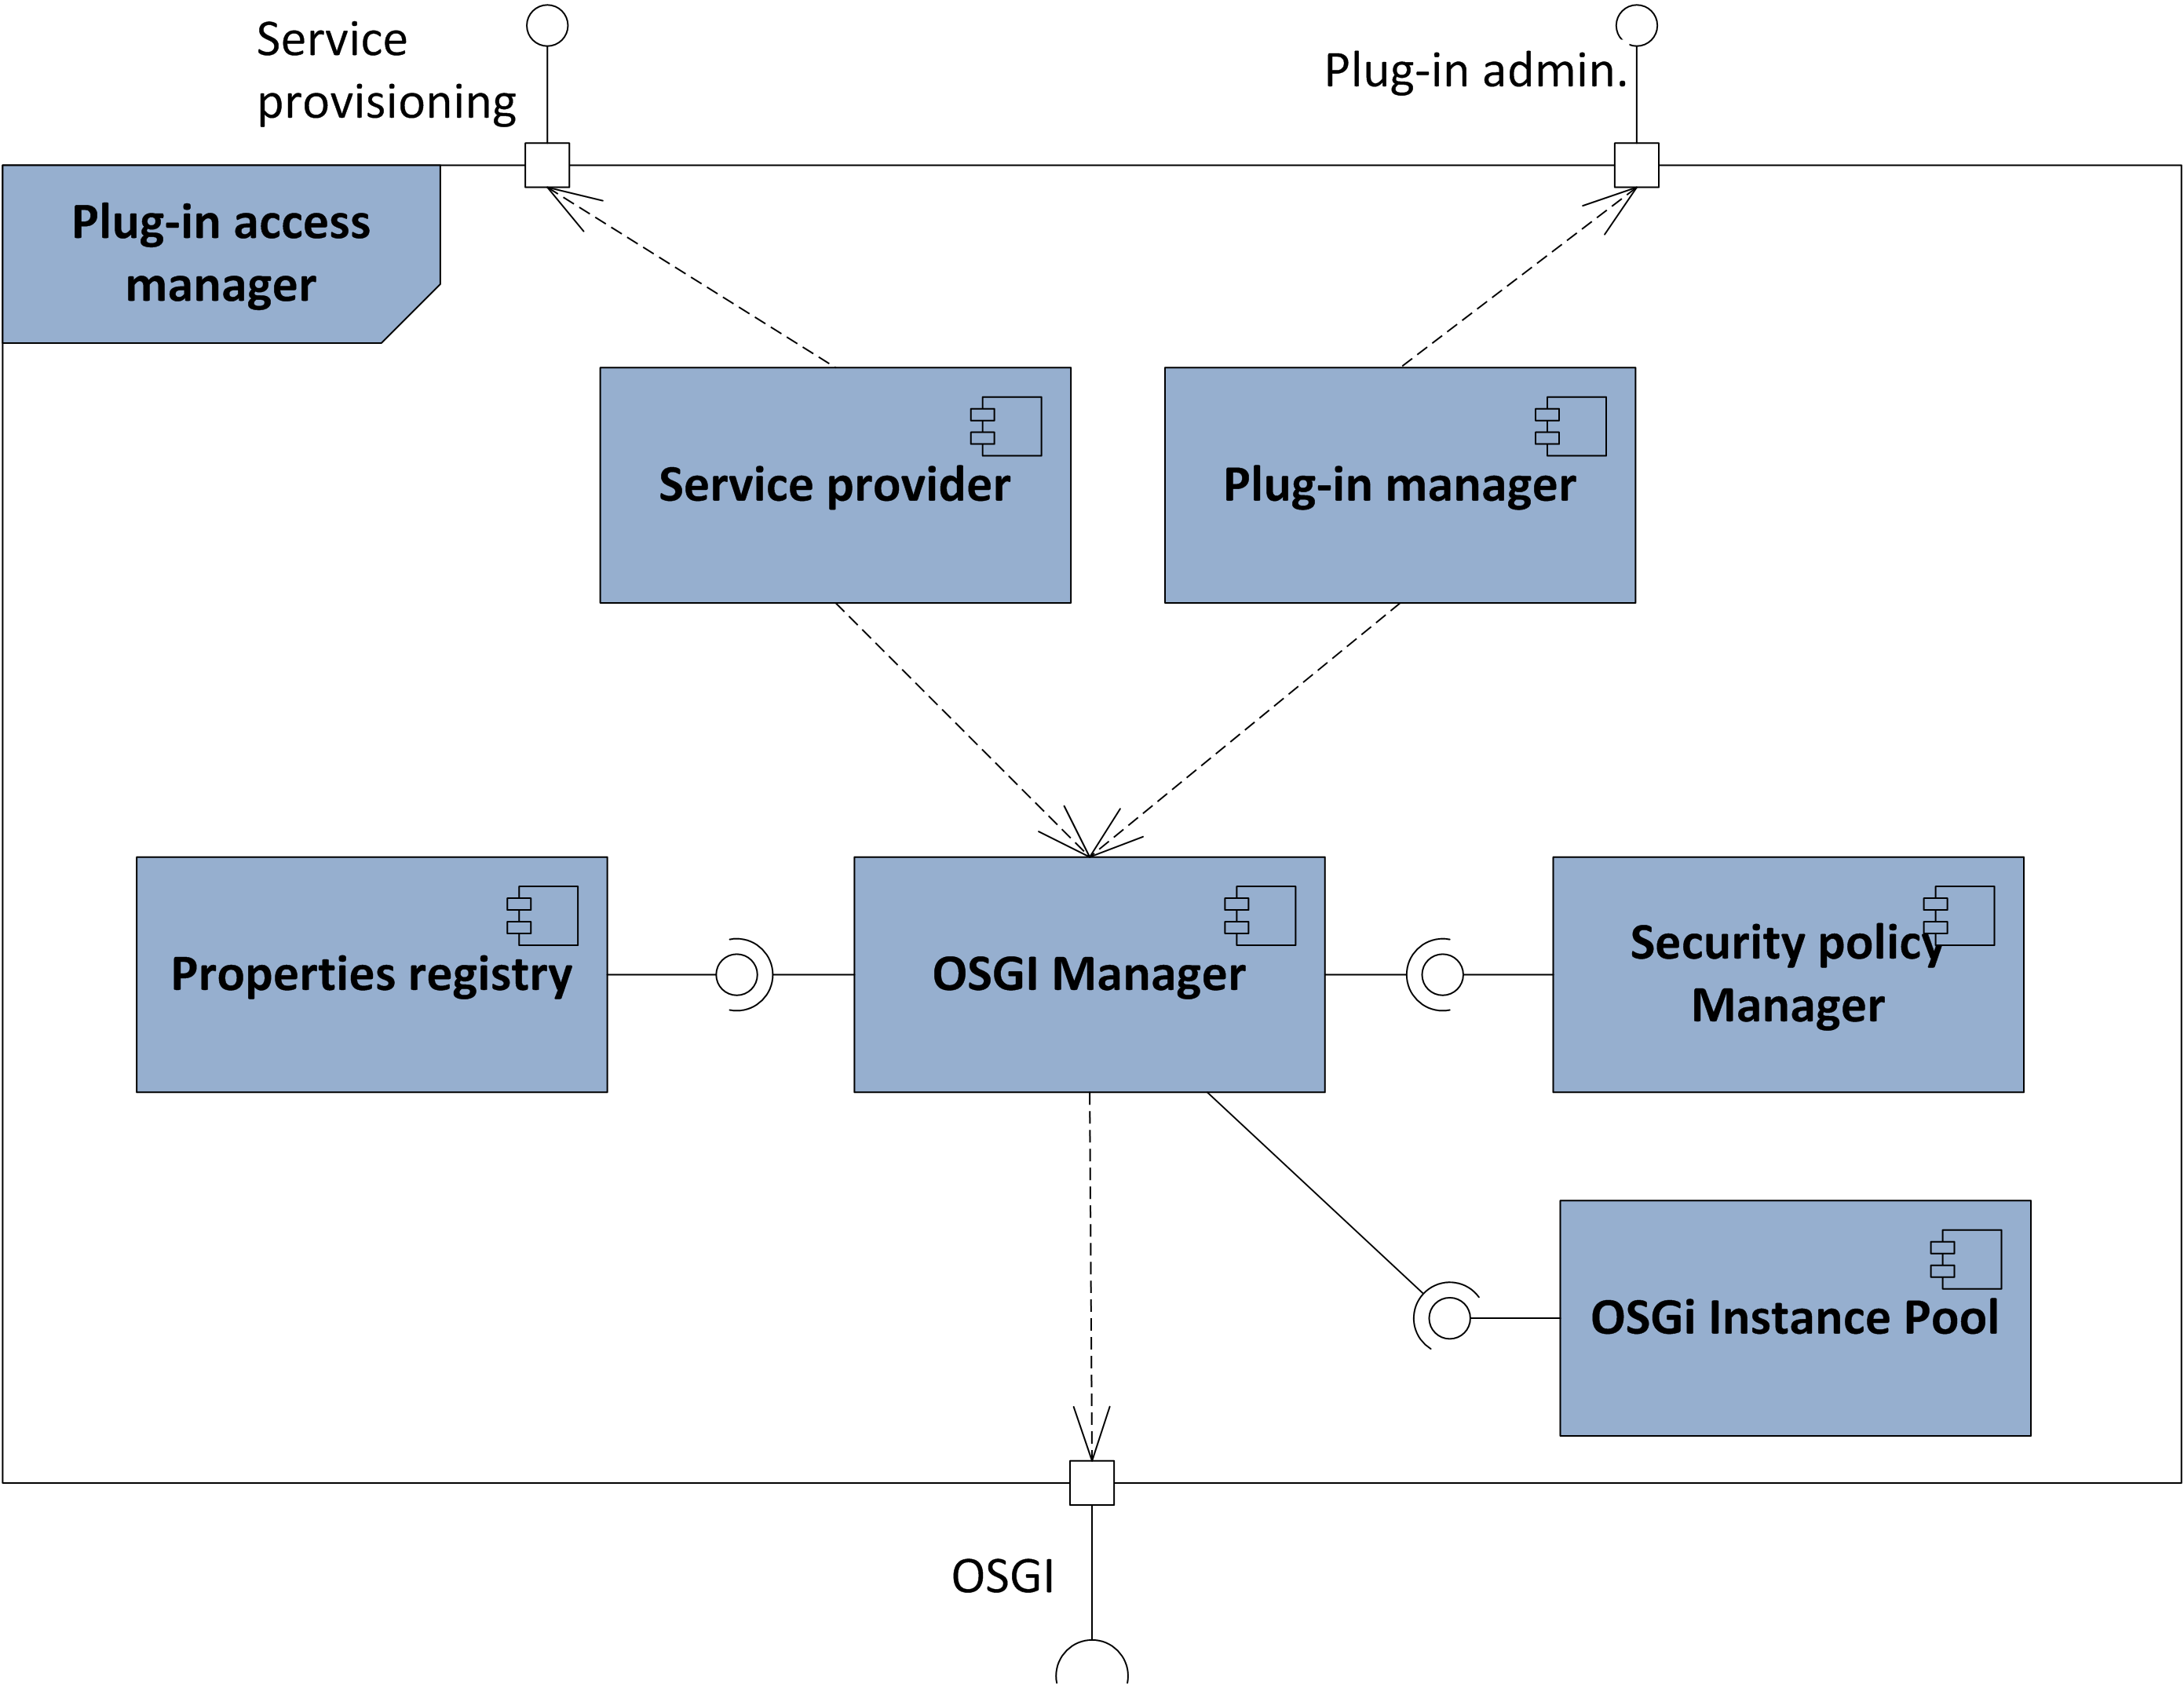
\includegraphics[scale=0.85]{plug-in/layers/access-func.png}
  \caption{Functional decomposition of the \textit{Plug-in access manager} component}
  \label{fig_access_func}
\end{figure}

\begin{itemize}

\item \textit{OSGI Manager} - This component manages the communication with the OSGI framework. It is responsible to start/stop the framework and monitor its life cycle. All needed properties for the framework operation are provided by the \textit{Properties registry} component. The OSGI Manager is also responsible to enforce the security policies by setting up the Security Manager options provided by the \textit{Security policy} component. It also acts as a level of abstraction over the plug-in engine and in case any change in future is required, this is the only component that will be affected. 

Starting an OSGi instance can be a time costly procedure especially when there are a lot of plug-in to be loaded. Therefore, in order to increase the performance of the system with the help of the \textit{OSGi Instance pool} component when an OSGi instance is no longer needed it is not destroyed but cached so that it can be later reused and not created again.

\item \textit{OSGi Instance pool} - based on the connection pool idea \cite{zhao2004design}, this component provides a cache of OSGi instances so that they can be reused when future interactions with the plug-ins are required.

\item \textit{Properties registry} - Keeps track of all common and user related options that are required for the correct operation of the OSGI framework. The main properties this component is responsible to provide are the paths to the plug-in storage space for each user. It has to make sure that this spaces are not overlapping. Additionally, it also provides information about the security policy that has to be applied to a particular user. 

\item \textit{Security policy manager} - This component is responsible to provide access to the security policies of U-Sem which define the operations that the custom code loaded by the framework is allowed to perform.

\item \textit{Plug-in manager} - This component is responsible to provide an API for the \textit{Application layer} components that enables them to perform plug-in management tasks.

\item \textit{Service provider} - This component is responsible to provide an API for the \textit{Application layer} components that enables them to access the services implemented by the loaded components in U-Sem.

\end{itemize}

\subsection{Concurrency view}
\label{sec:pluginConcur}

This section describes the concurrency structure of U-Sem. We show how functional elements map to concurrency units(processes, process groups and threads) in order to clearly identify the parts of the system that can work concurrently. We also show how this parallel execution is coordinated and controlled.

\begin{figure}[h!]
  \centering
  	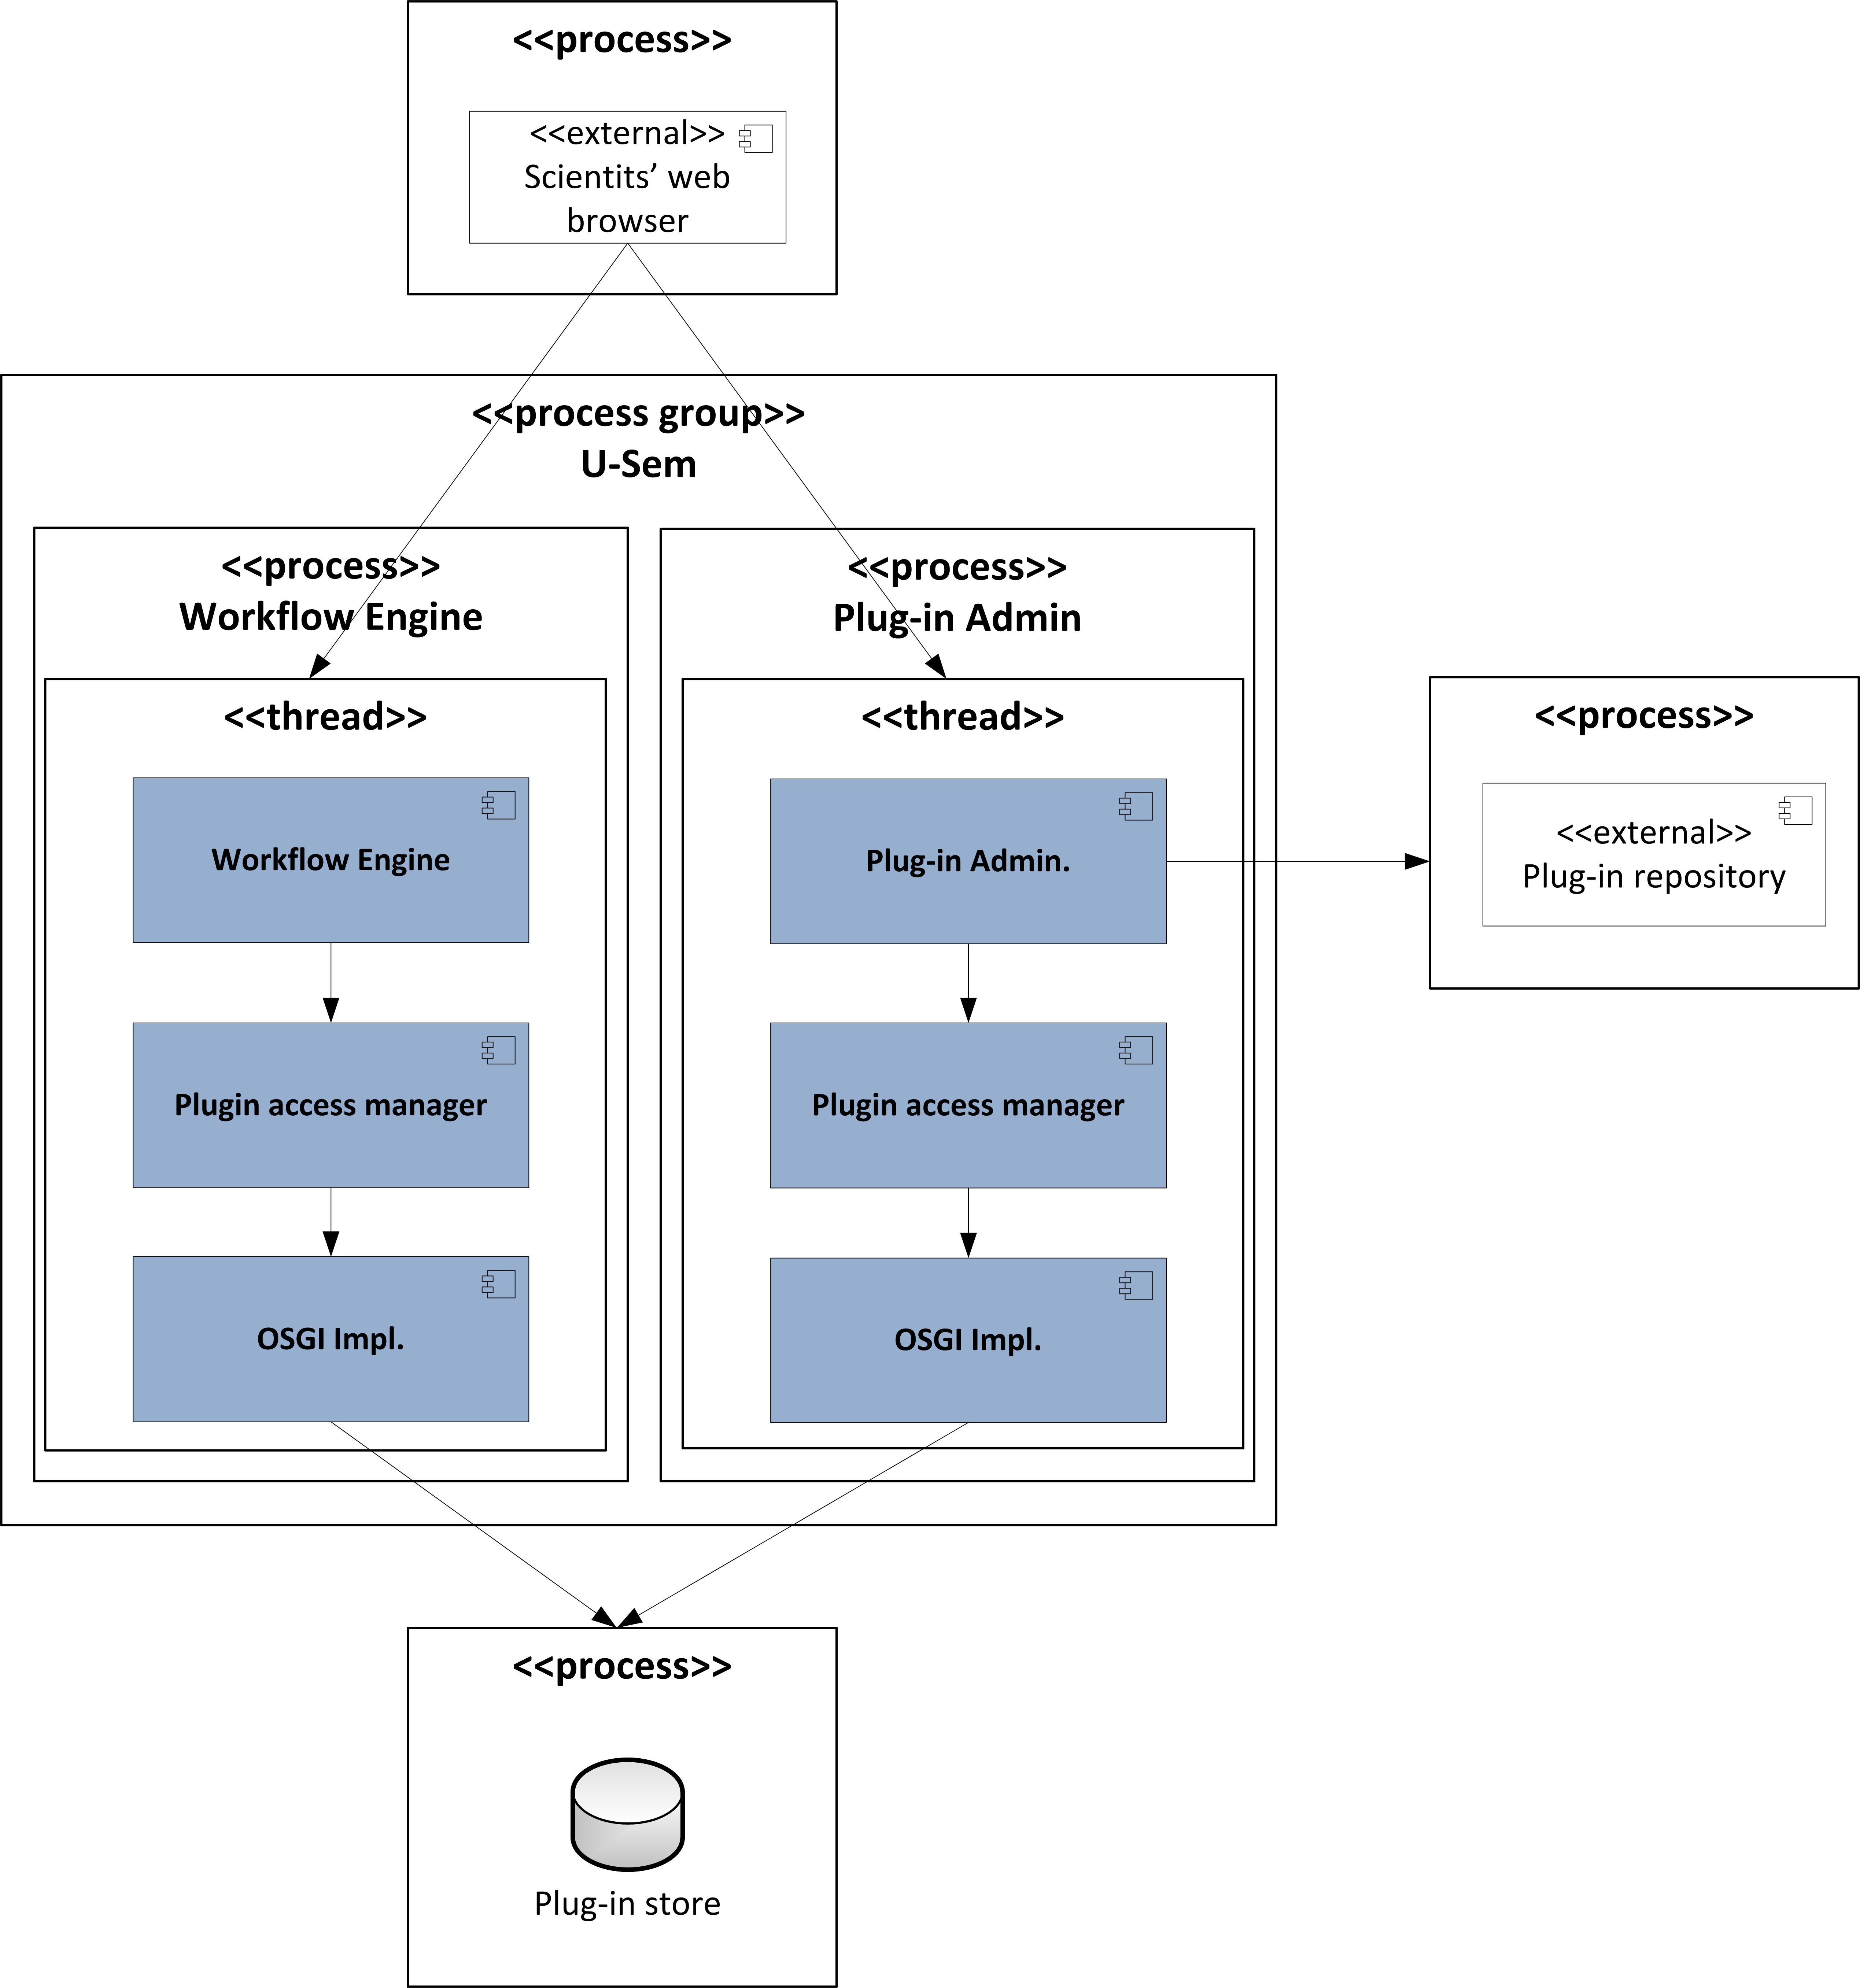
\includegraphics[scale=0.70]{plug-in/layers/concur.png}
  \caption{Diagram illustrating the concurrency model of the solution}
  \label{fig_conc}
\end{figure}

Figure \ref{fig_conc} illustrates the concurrency organization of U-Sem. The main functionality of the system is situated in the U-Sem process group. All U-Sem processes and all external processes(Plug-in repository) including the Database process operate concurrently. The main processes wait for requests from the user(web browsers and/or other systems). Each request is processed in separate thread depending on its type(workflow or plug-in management related tasks). As a result, multiple client requests can be handled simultaneously. The main idea behind this design is to separate the workflow and the Plug-in administration functionality into separate processes which enhances loose coupling and, hence, improves maintainability and simplifies upgrades to new versions of the workflow engine. Additionally, if in future there is a need for higher performance the workflow process can be replicated without affecting the plug-in administration functionality. This organization, however, also introduces some problems that have to be solved:

\subsubsection{Problems}

The first problem lies in the fact that plug-in installation (plug-in admin.) and loading of plug-ins (workflow engine) are two actions that are completely independent from each other. Therefore, if the wokrflow engine tries to load the plug-ins when the plug-in admin. is in the middle of installation of plug-ins then the plug-ins may fail to load or load incorrectly. 

Secondly, as discussed in the previous section the system keeps a pool with the OSGi instances so that they can be reused instead of loaded from scratch. However, whenever a plug-in is installed or removed these cached instances become obsolete and have to be discarded. In order to do that, the plug-in admin. has to notify the workflow engine for the change in the plug-ins which is a problem when the two components are in separate processes.

\subsubsection{Solution}

In order to solve the first problem we propose a solution that is based on synchronization between the processes. The solution is based on the \textit{Reader-Writer Lock} idea. It extends mutual exclusion locks by enabling concurrent read access to a shared resource but requires exclusive access for write operations \cite{lev2009scalable}.

Our solution maps to the \textit{Reader-Writer Lock} idea as follows:
\begin{itemize}
	\item The shared resource is the plug-in storage of an engineer.
	\item The workflow engine acts as reader of the shared resource.
	\item The plug-in administration acts as writer of the shared resource.
\end{itemize}

As a result, when a change to the plug-ins is needed it is executed exclusively and any components that want to load the plug-ins have to wait until the change is applied. Therefore, the workflow engine is protected against loading the plug-ins while they are inconsistent. This approach also brings a performance benefit since loading plug-ins is not exclusive and can be done simultaneously by many components. 

The standard \textit{Reader-Writer Lock} in Java, however, works only within the virtual machine \footnote{http://docs.oracle.com/}. In our case we have to synchronize entire processes. Our research showed that there are already existing tools that provide this functionality \cite{hernane2012dynamic}. The tool that is used in the proposed solution is Terracotta \footnote{http://terracotta.org/}. It introduces a process that is responsible for the lock and the other processes communicate with it in order to obtain the lock and use the resources.

In order to solve the second problem we extend the architecture by providing mechanism for inter-process communication in order to enable the plug-in admin. to notify all processes for any updates so that they can clean their caches. The general idea is that all components that maintain caches register to receive updates when plug-ins change. Whenever this happens all registered components are notified using a broadcast protocol \cite{joseph1988reliable}. Our research showed that the Terracotta system that we used to solve the first problem also provides implementation of a broadcast protocol. Therefore, when a workflow engine loads the plug-ins it contacts the Terracotta process and registers itself for updates regarding the plug-ins. When an engineer removes or installs a plug-in the plug-in admin. contacts the Terracotta process which then notifies all the registered clients.

Having presented the most important features of the architecture of the solution we continue by discussing its implementation in next section. 


\section{Implementation}
\label{sec:implPlugin}

We implemented the proposed architecture in order to evaluate its applicability and capabilities. This section describes the main steps we performed during the implementation of the system.

First, we had to choose which OSGI implementation to use. Nowadays there are several vendors that provide implementations. The most popular are: Equinox\footnote{Equinox. http://www.eclipse.org/equinox}, Felix\footnote{Apache felix. http://felix.apache.org} and Knopflerfish\footnote{Knopflerfish. http://www.knopflerfish.org} \cite{tavares2008gentle}. Theoretically, they all strictly implement the OSGI standard and therefore, there should be little difference. However, we choose Equinox because it seemed more matured and more widely used compared to the others. Moreover, Equinox is highly integrated in the popular Eclipse IDE. This enables engineer to use the out-of-the box functionality for creating plug-ins in Eclipse.

Secondly, we had to decide the points where U-Sem can be extended by providing custom functionality from plug-ins. Looking at the requirements, we identified that engineer has to be able to provide custom workflow functions and entire workflow definitions. As explained earlier, in OSGI this points for extension are represented as java interfaces or classes. For providing custom workflow functions engineers have to use the \textit{RGLFunction} class. The situation with the workflows was more complicated since they are represented as resource(xml) files. OSGI does not provide direct way for providing custom resource files from plug-ins. In order to overcome this problem, we defined a new class called \textit{WorkflowTemplate} which acts as a bridge and enables the workflow engine and other components to access workfow definition files provided by custom plug-ins.

\begin{figure}[h!]
  \centering
  	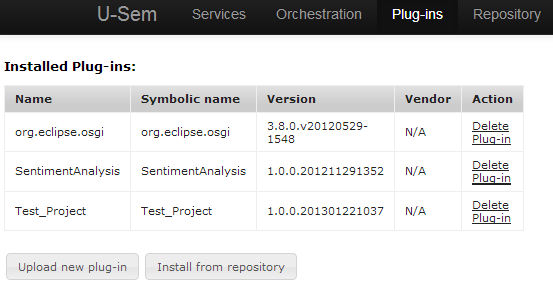
\includegraphics[scale=0.70]{plug-in/ui/list.png}
  \caption{User interface for plug-in management.}
  \label{list_ui}
\end{figure}

Next, we provided a very simple implementation of a plug-in repository. It represents a simple web application which stores the plug-ins locally into the file system of the web server where it is deployed. The implementation provides REST interface for retrieving the list of available plug-ins and providing the contents of a selected plug-in. We also implemented very simple user interface which enables engineers to upload their plug-ins. 


\begin{figure}[h!]
  \centering
  	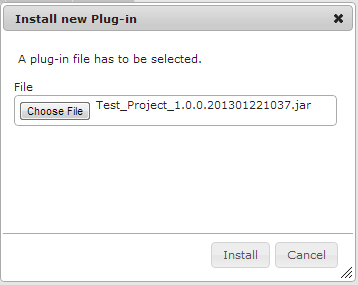
\includegraphics[scale=0.6]{plug-in/ui/upload.png}
  \caption{User interface for uploading and installing plug-ins in U-Sem.}
  \label{upload_ui}
\end{figure}

We continued by implementing all the components defined in the proposed architecture of U-Sem. In order to implement the endpoints(user interface) we used the jQuery UI\footnote{http://jqueryui.com/} and Bootstrap\footnote{http://twitter.github.com/bootstrap/} technologies. Figure \ref{list_ui} represents the endpoint for viewing all installed plug-ins. The detailed information about all installed plug-ins is represented in a table. Each row has a "Delete" button which provides access to the functionality for removing plug-ins. At the bottom of the view, there are two buttons that lead to the endpoints for uploading a plug-in depicted in figure \ref{upload_ui} and the endpoint for browsing and installing functionality from the repository depicted in figure \ref{repo_ui}.

\begin{figure}[h!]
  \centering
  	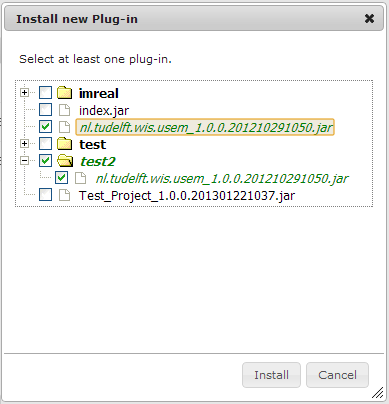
\includegraphics[scale=0.6]{plug-in/ui/repo.png}
  \caption{User interface for browsing and installing plug-ins from the plug-in repository.}
  \label{repo_ui}
\end{figure}

We also constructed a Maven build script that packs all source files into deployable components(war files) that can be directly deployed to a web server. The entire system is built into the following deployable files:
\begin{itemize}
	\item \textit{rdfgears.war} providing the workflow engine.
	\item \textit{pluginmanagement.war} providing the functionality for managing plug-ins.
	\item \textit{localPluginRepo.war} providing the implementation of the simple plug-in repository.
\end{itemize}


\section{Evaluation}
\label{sec:evalPlugin}

After successfully implementing the system, in this section we evaluate whether the system actually solves the problems identified in Section \ref{sec:problemDefPlugin}. In order to do the evaluation we asked engineers to use the new solution to implement real world user modelling services and asked them to comment on the problems the solution is designed to solve. The following is summary of the engineers feedback:

\begin{itemize}
	\item The new solutions saves time and efforts to the engineers. This is because the process of adding functional components to U-Sem is significantly simplified. Engineers no longer have to modify, build and deploy the workflow engine every time they execute the task. Instead they can develop their functional components separately from the wokflow engine and install them when needed. This processes are also automated and requires almost non overhead work from the engineers. 
	
	\item Engineers reported that the time needed for training new engineers to work with the system is significantly reduced. Because of the simplified process they do not have to learn how to check out, modify, build and deploy the workflow engine. Instead they only have to learn how to build the plug-ins and install them to the system using the tutorial presented in Appendix \ref{cha:tutorial}.
	
	\item Engineers no longer disrupt each others work because adding functional components to the system is performed in isolation for each user and there is also no need for restarting the system. 
	
	\item The versioning issue explained in Section \ref{sec:problemDefPlugin} is no longer a problem because engineers deploy and use the plug-ins in isolation between each other and there is no way that one engineer can modify the plug-ins of another.
	
	\item Engineers also reported that the implementations of the functional components are no longer so tightly coupled between each other because the source code is no longer freely available as part of the workflow engine. It is now owned by the engineers themselves and using the information hiding mechanisms of OSGi they can define more precisely which part of their code can be accessed and which not.
	 
\end{itemize} 

Analysing this feedback we can conclude that we have solved the problems defining the Plug-in Environment feature and the designed and implemented system is capable of serving its intended purpose. As most scientific works there is still a place for improvement in this one as well. In next section we discuss possible directions for future work regarding the feature.


\section{Limitations and Future Work}
\label{sec:limitsPlugin}

In this section we identify the limitations of the proposed architecture and we also suggest approaches that can be used to overcome these limitation in the future. We have identified two groups of limitations concerning U-Sem. The first group represents the limitations that are inherited from the usage of OSGI. The second one consists of the limitations concerning the rest of the U-Sem's architecture.

Most of the limitations concerning OSGI originate from the potential vulnerabilities of running external code which the security mechanism fails to fully address. The authors of \cite{parrend2009security} have studied in details the potential vulnerabilities of OSGI. These vulnerabilities can be grouped into the following categories:

\begin{itemize}

	\item \textit{Vulnerabilities on operating system level} - This kind of vulnerabilities result from the fact that it is possible that a plug-in runs malicious native code using the Java JNI. Native code is not managed by the JVM and thus, the security policy is not applied. \cite{sun2012jvm} proposes a portable solution for sandboxing of Java's Native Libraries without modifying the JVM's internals which might be used for overcoming these vulnerabilities.
	
	\item \textit{Vulnarabilities on OSGi platform level} - This kind of vulnerabilities are related to weaknesses in the OSGi run-time. \cite{parrend2009security} suggests an approach for overcoming them by adding additional security checks in the OSGi implementation.
	
	\item \textit{Vulnarabilities on JVM level} - This vulnerabilities can be further divided into categories \cite{geoffray2009jvm}: 
	
	\begin{itemize}
		\item \textit{lack of isolation} - Even though components for each user are loaded through separate OSGI instances, on JVM level \textit{java.lang.Class} objects and static variables are shared by all plug-ins. A malicious bundle can interfere with the execution of other bundles by altering static variables or obtaining lock on shared objects.
		
		\item \textit{lack of resource accounting} - In OSGI each plug-in is loaded with a separate class loader. However, JVM does not perform resource monitoring on a per class loader basis. Therefore, in case of the overuse of resources(CPU, memory), it is impossible to identify the faulty bundle and stop its execution.
		
		\item \textit{failure to terminate a bundle} -  If the system recognizes a bundle as misbehaving and wants to stop its
execution it might fail if methods of the bundle are being executed at that point. Moreover, a malicious code can run an infinite loop in the Java \textit{finalize} method and thus prevent memory reclamation.
		
	\end{itemize}
	
	\cite{geoffray2009jvm} proposed and approach for overcoming these vulnerabilities. They have designed I-JVM, an extension of the Java Virtual Machine which provides functionality for component isolation and termination in OSGi.
	
\end{itemize}

At this point, U-Sem is aimed to be used by engineers from a single organization. Therefore, the components will only be reused within the organization which limits the possibility for any external person adding plug-ins into the system. Therefore, exploitation of the discussed vulnerabilities on purpose is not so likely. Therefore, we believe that this limitations does not pose a significant threat for U-Sem. However, all these vulnerabilities has to be addressed if in future the system is to be extended to enable access from unverified engineers. 
